% !TEX root = ../main.tex
% chktex-file 21
\section{Optimizing Training}%
\label{sec:params}

Now follows an overview of approaches to speed up the training process.
We will discuss four approaches:
\begin{enumerate}
	\item A general purpose method that combines subsampling with bootstrapping.
	\item An iterative method to select the optimal subsample size during gradient descent.
	\item Improving the quality of subsampling for logistic regression by weighing the samples.
	\item Speeding up the training of SVMs via \(k\)-means clustering.
\end{enumerate}

\subsection{Bag of Little Bootstraps}%
\label{sec:params:blb}

The first approach we will discuss is called \textit{Bag of Little Bootstraps}~(BLB)~\cite{Kleiner2011}.
It combines subsampling with bootstrapping and is particularly well suited for parallelized implementations.

In the context of Big Data training typically cannot be performed on the entire dataset.
A na{\"\i}ve way to solve this problem is to simply train on a random \(b\) out of \(n\) subsample of the data \(\Dtrain = \{X_1, \dots, X_n\}\).
This approach is highly sensitive to noise in the training dataset, especially if \(b \ll n\).
To overcome this problem bootstrapping can be used.
The regular \(n\) out of \(n\) bootstrapping technique for variance reduction is not suitable for big datasets because it uses \(63\%\) of the training data on average.
However the \textit{\(b\) out of \(n\) bootstrapping} (BOFN) approach can in principle be applied.
It uses \(s\) samples \(\{\check{X}^{(i)} = (\check{X}_1^{(i)}, \dots, \check{X}_b^{(i)})\, |\, 1 \leq i \leq s\}\) of \(b\) datapoints each.
Since this approach independently learns \(s\) hypotheses \(h_i\) on small datasets \(\check{X}^{(i)}\), their parameterizations \(\theta_i\) tend to have large confidence intervals.
Because of that, the quality of the combined hypothesis is strongly dependent on \(b\).
BLB reduces this dependence.

\subsubsection{Intuition}%
\label{sec:params:blb:intuition}

BLB is a simple extension of BOFN that is consistently more robust regarding the choice \(b\) across datasets.
The basic idea is to add another sampling step.
BLB uses each subsample \(\check{X}^{(i)}\) as a seed for \(n\) out of \(b\) sampling.
This yields bigger resamples \(\{X^{*(i, k)} = (X_1^{*(i, k)}, \dots, X_n^{*(i, k)})\, |\, 1 \leq i \leq s, 1 \leq k \leq r\}\) that each contain at most \(b\) different elements.
Training is then run on the resamples \(X^*\) instead of the small seed samples \(\check{X}\).
The learned hypothesis parameterizations are finally combined to a single hypothesis parameterization \(\theta^*\) via a model specific combination function, e.~g.\@ by simply taking the average.
Figure~\ref{fig:blb:overview} illustrates those steps.
\begin{figure}
	\centering
	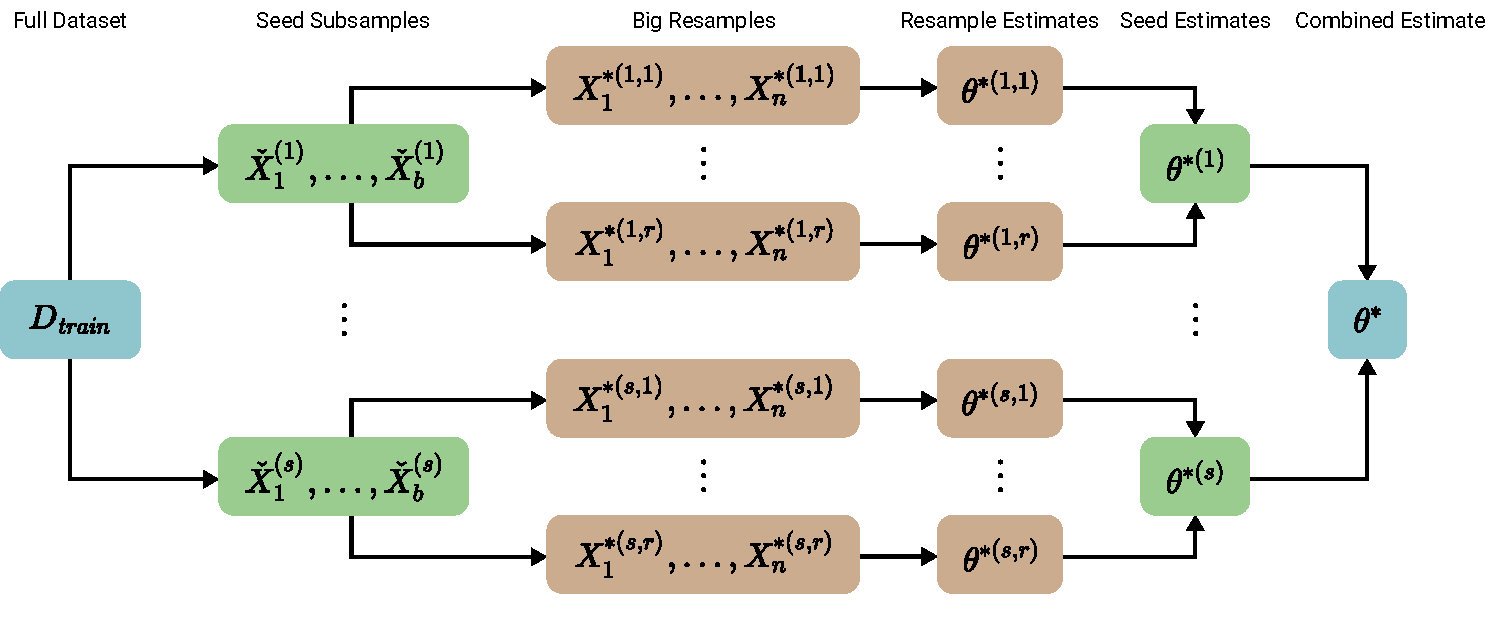
\includegraphics[width=\linewidth]{gfx/blb/overview.pdf}
	\caption{Overview of the steps of BLB.}\label{fig:blb:overview}
\end{figure}

Even though BLB trains classifiers on resamples of size \(n\) its time and space complexity effectively still depends on \(b\), not \(n\).
This is because each resample \(X^*\) only contains at most \(b\) different elements which means that it can be efficiently represented by a list of \(b\) multiplicity counts \((c_1, \dots, c_b) \in \mathbb{N}^b\), i.~e.\@ \(\mathit{space} = \mathcal{O}(b \log n)\).
Training on such a dataset is equivalent to training on a dataset of size \(b\) with weights \(w_i = \frac{c_i}{n}\).
Since most commonly used classifiers support weighted samples, BLB is widely applicable and, because of the independence of the resamples, easily parallelizable.

\subsubsection{Evaluation}%
\label{sec:params:blb:eval}

\begin{figure}
	\begin{subfigure}{0.5\textwidth}
		\centering
		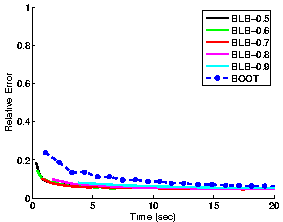
\includegraphics[width=0.9\linewidth]{gfx/blb/time1.pdf}
	\end{subfigure}
	\begin{subfigure}{0.5\textwidth}
		\centering
		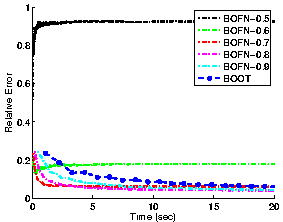
\includegraphics[width=0.9\linewidth]{gfx/blb/time2.pdf}
	\end{subfigure}
	\caption{
		Comparison of BLB and BOFN with regular \(n\) out of \(n\) bootstrapping (BOOT) using logistic regression.
		The error on the average of all sample hypotheses that were computed within a given time is shown.
		\(b = n^\gamma\) for multiple values of \(\gamma \in [0, 1]\) is used.
	}\label{fig:blb:eval}
\end{figure}

\subsection{Subsample Size Selection for Gradient Descent}%
\label{sec:params:samplesize}

Next we will discuss gradient descent based optimization.
The sample size \(S\) that describes the number of datapoints that are considered in a single gradient descent step heavily influences the optimizer's behavior:
\begin{itemize}
	\item In the stochastic approximation regime small samples, typically \(S = 1\), are used. This causes fast but noisy steps.
	\item In the batch regime large samples, typically \(S = |\Dtrain|\), are used. Steps are expensive to compute but more reliable.
\end{itemize}
Both extremes are usually not suitable for Big Data applications.
Very small samples cannot be parallelized well, making them a bad fit for the compute clusters that are typically available nowadays.
The gradients for very big samples however are often too slow to compute.
\(S\) should ideally lie somewhere in between.

\citet{Byrd2012} describe an iterative algorithm that dynamically increases \(S\) as long as this promises to significantly reduce the gradient noise.

\subsection{Subsampling for Logistic Regression}%
\label{sec:params:osmac}

Subsampling usually increases the mean squared error (MSE) of the resulting hypothesis compared to one that is trained on the full dataset.
OSMAC~\cite{Wang2017} is a method that improves upon na{\"\i}ve subsampling by weighing the samples.

\textit{TODO:\@ explain OSMAC}

\subsection{SVM-KM}%
\label{sec:params:svmkm}

To speed up the training of SVMs \citet{Almeida2000} proposed a simple method that reduces the dataset size via \(k\)-means clustering.
It can be described as a three-step procedure:
\begin{enumerate}
	\item Group the training samples \(\Dtrain\) into \(k\) clusters \(C_1, \dots, C_k\) with centers \(c_1, \dots, c_k\) where \(k\) should be determined via hyperparameter optimization.
	\item Check for each cluster \(C_i\) whether all associated datapoints belong to the same class, i.~e.\@ \(\exists\, z \in \{+1, -1\}: \forall (x, y) \in C_i: y = z\).
		If yes, all datapoints in \(C_i\) are removed from \(\Dtrain\) and replaced by \(c_i\).
		If not, they are kept in the dataset.
		The intuition behind this is that clusters with points from multiple classes might be near the decision boundary so they are kept to serve as potential support vectors.
	\item Finally standard SVM training is performed on the reduced training dataset.
\end{enumerate}

\subsubsection{Evaluation}%
\label{sec:params:svmkm:eval}

\textit{TODO}
